%%%%%%%%%%%%%%% Experimental Comparison %%%%%%%%%%%%
\subsubsection{Experimental Comparison}
Now that we have made some comparisons of our results with theoretical models and equations. It is the next step to validate our results by comparing them with data obtained from previous experimental studies. To achieve this, we will be using an article published by Hammad et al.\cite{hammad_ötügen_arik_1999}. In their study, they also observed and analized the flow of a fluid through an expanding pipe.

\begin{figure}[H]
 \centering
\begin{subfigure}{.7\textwidth}
  \centering
  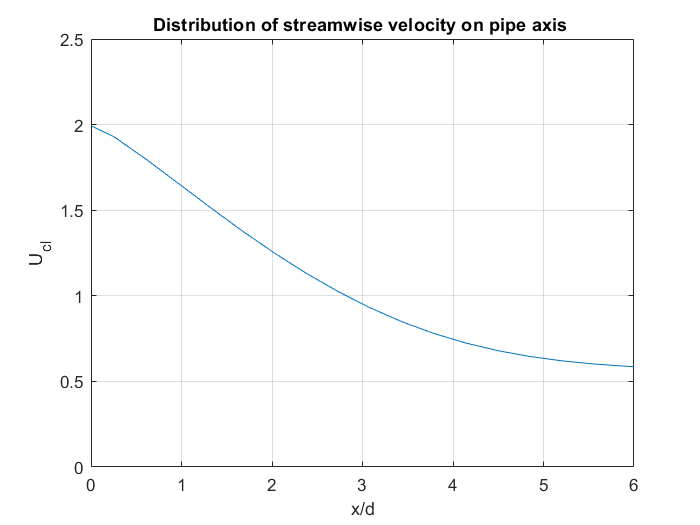
\includegraphics[width=.7\linewidth]{images/task1/x_d_norm.png}
  \caption{Distribution of streamwise velocity on pipe axis of ANSYS data.}
  \label{fig:x_d_norm}
\end{subfigure}%

\begin{subfigure}{.8\textwidth}
  \centering
  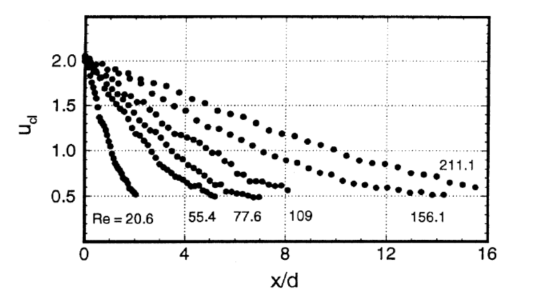
\includegraphics[width=.9\linewidth]{images/task1/x_d_norm_actual.png}
  \caption{Distribution of streamwise velocity on pipe axis from Hammad et al.\cite{hammad_ötügen_arik_1999}}
  \label{fig:x_d_norm_actual}
\end{subfigure}

\caption{Streamwise Velocity Comparison}
\label{fig:xd_norm}
\end{figure}

\noindent Figure \ref{fig:xd_norm} shows the similarities with data from our simulation and the data provided by \cite{hammad_ötügen_arik_1999}. While their chart contains data points from 6 different flows with different Reynolds numbers, the one which $Re = 55.4$ corresponds to our MATLAB plot that is shown above with very little error. This distribution makes sense since the fluid enters the second pipe with the highest velocity that is obtained from the equation \ref{eq:hagen} and that value corresponds to twice of the average velocity of the fluid. However, as the fluid moves deeper into the second pipe, the velocity at the centerline drops to around half of the average velocity.\\


\noindent Moreover, Hammad et al. provides velocity vectors for the case of $Re = 55.4$ throughout the length of the wider pipe. Once we obtain the velocity vector plots from ANSYS Fluent ourselves, a comparison can be made between our simulated data and their experimental data. 

\begin{figure}[H]
 \centering
\begin{subfigure}{.8\textwidth}
  \centering
  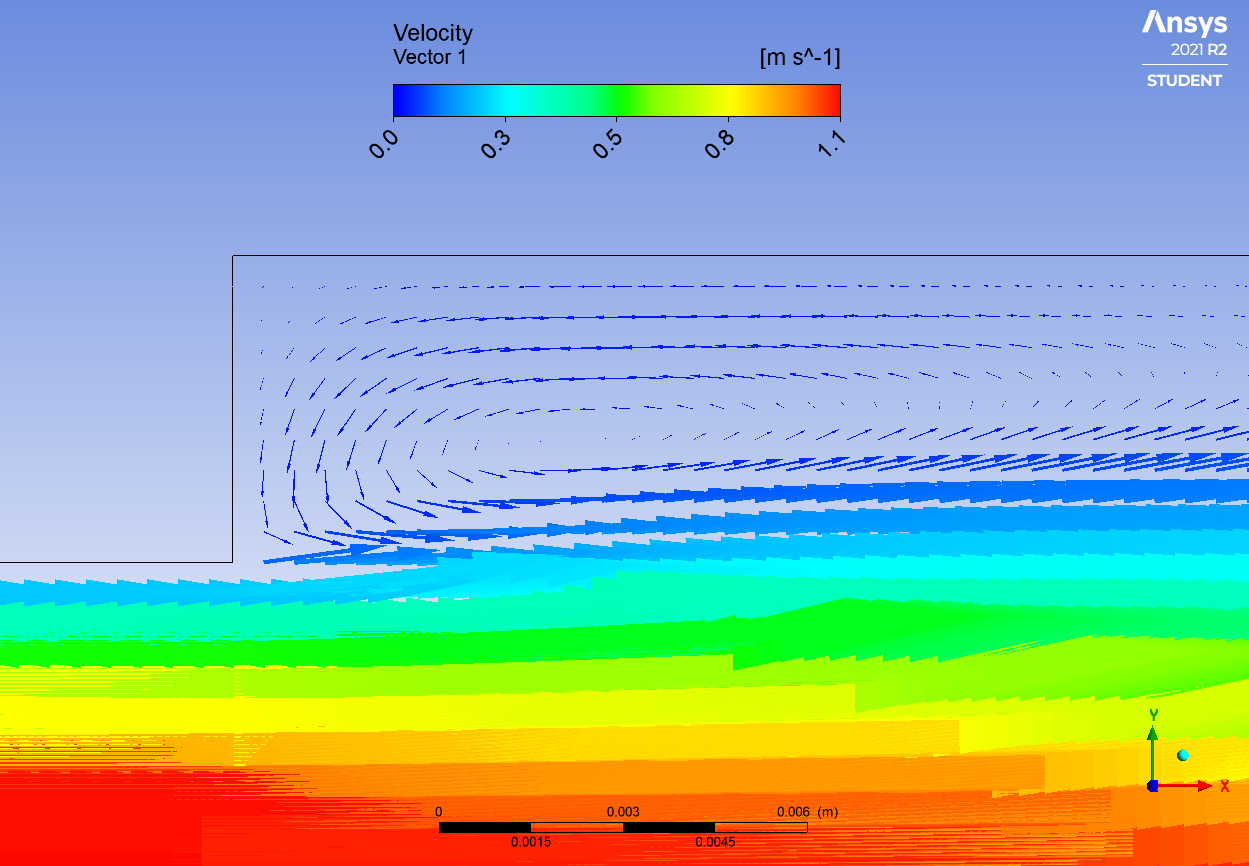
\includegraphics[width=.8\linewidth]{images/task1/vectors.png}
  \caption{Upscaled velocity vectors at the expansion.}
  \label{fig:vel_vel1}
\end{subfigure}%
\hfill
\begin{subfigure}{.8\textwidth}
  \centering
  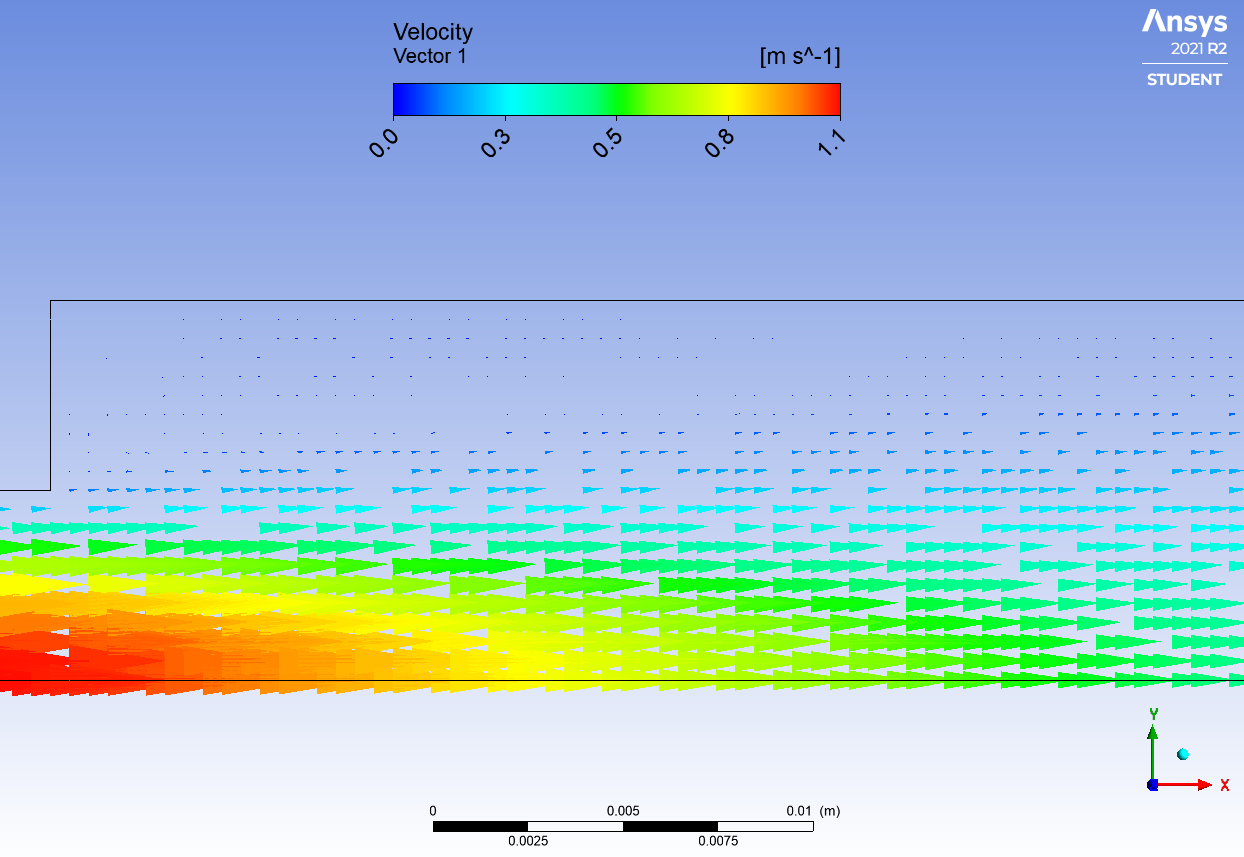
\includegraphics[width=.8\linewidth]{images/task1/vectorsplot.png}
  \caption{Velocity vectors at the expansion.}
  \label{fig:vel_vel2}
\end{subfigure}
\hfill
\begin{subfigure}{.8\textwidth}
  \centering
  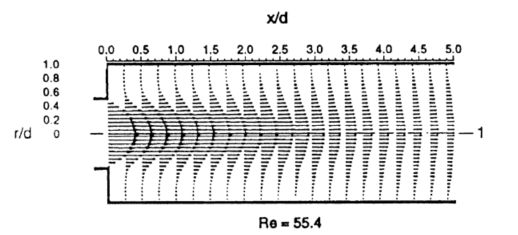
\includegraphics[width=.9\linewidth]{images/task1/vel_vectors.png}
  \caption{Measured velocity vectors from Hammad et al.\cite{hammad_ötügen_arik_1999}}
  \label{fig:vel_vel_measured}
\end{subfigure}

\caption{Streamwise Velocity Comparison}
\label{fig:vel_vec_comp}
\end{figure}

\vspace{0.5cm}
\noindent As can be seen from Figure \ref{fig:vel_vec_comp}, the measured values from the study and our Fluent simulation are in agreement. They both have maximum magnitude at the centerline and the magnitude gets smaller as the position of the vector gets farther away from the centerline. Also, as $x/d$ increases, magnitude of the vectors on the centerline decreases for both cases.
\\

\noindent Another aspect that was observed and modeled by Hammad et al. is the reattachment length of around the recirculation zone. In our case, the reattachment length is found looking at the streamlines and finding the point at which a streamline connects to the wall. The part before the reattachment point is called the recirculation zone. For this experiment, reattachment points have been found and plotted for 4 different $Re$ values. The change in the $Re$ values are made possible by changing the inlet velocities. Tested $Re$ values are 30, 55.4, 100 and 150.\\



\noindent The determination of the locations of the reattachment points is shown in Figure \ref{fig:reattach}. For all different cases, finding the reattachment point required tinkering with the number of streamlines to be drawn since in some cases. This was due to the fact that the location of the reattachment point was dependent on the concentration of the streamlines. The crosshairs and highlighted points on Figure \ref{fig:reattach}, depict the decided positions of reattachment points.


\begin{table}[H]
\caption{Reattachment lengths for Reynolds numbers}
\centering
\begin{tabular}{c|c}
\hline
Reynolds Number & Reattachment Length (m) \\ \hline
30              & 0.0141                  \\
55.4            & 0.0236                  \\
100             & 0.0430                  \\
150             & 0.0681                 
\end{tabular}
\end{table}

\noindent These numbers do follow the trendline that Hammad et al. has shown in their study and this can be shown by plotting our points over their chart, which can be seen from Figure \ref{fig:reattach_plot}. In this plot, our data points are shown with green circles. 

\begin{figure}[H]
    \centering
    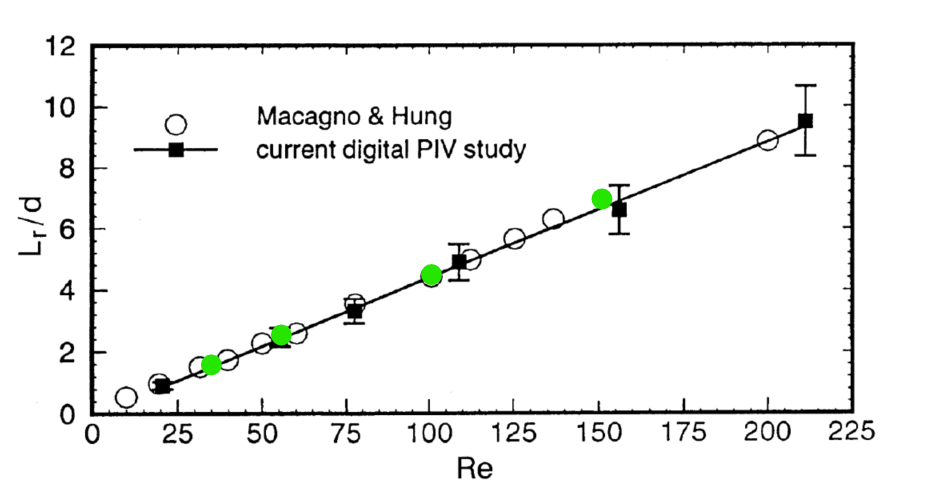
\includegraphics[width=14cm]{images/task1/reattach_plot.png}
    \caption{Plot of simulated reattachment lengths over the model of Hammad et al.}
    \label{fig:reattach_plot}
\end{figure}



\begin{figure}[H]
 \centering
\begin{subfigure}{.5\textwidth}
  \centering
  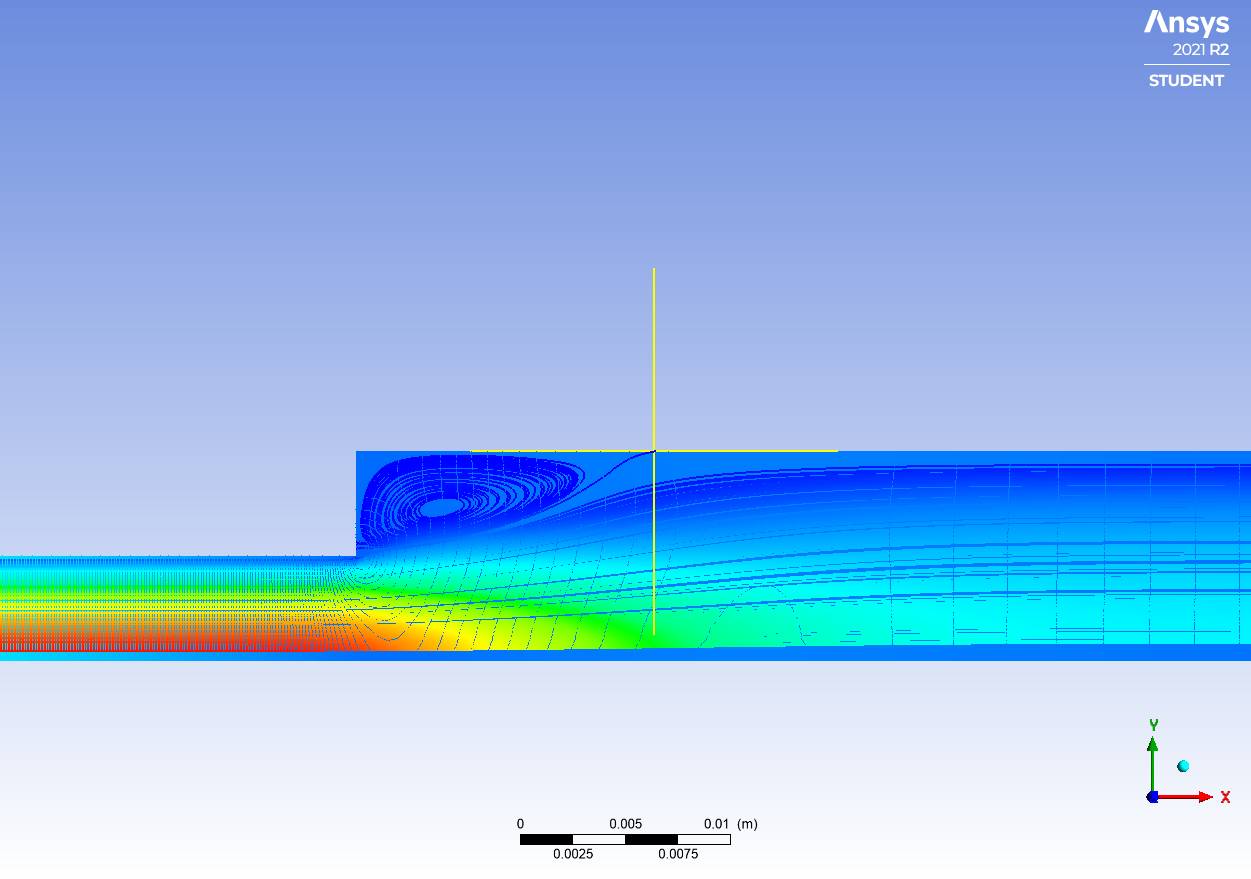
\includegraphics[width=.95\linewidth]{images/task1/030_attachement_0_0141.png}
  \subcaption{}
  \label{fig:reat_a}
\end{subfigure}%
\hfill
\begin{subfigure}{.5\textwidth}
  \centering
  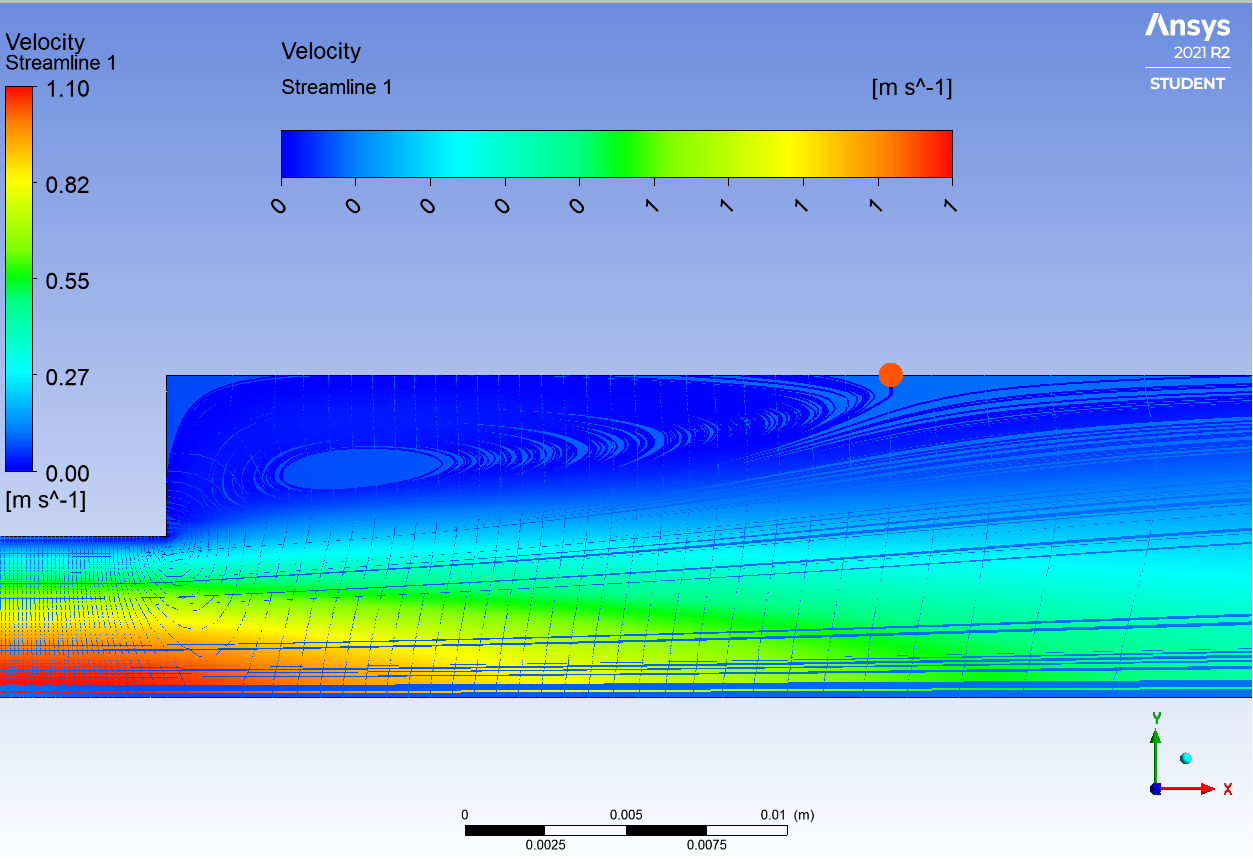
\includegraphics[width=.95\linewidth]{images/task1/0554_attachement_0_0236.png}
  \subcaption{}
  \label{fig:reat_b}
\end{subfigure}
\hfill
\begin{subfigure}{.75\textwidth}
  \centering
  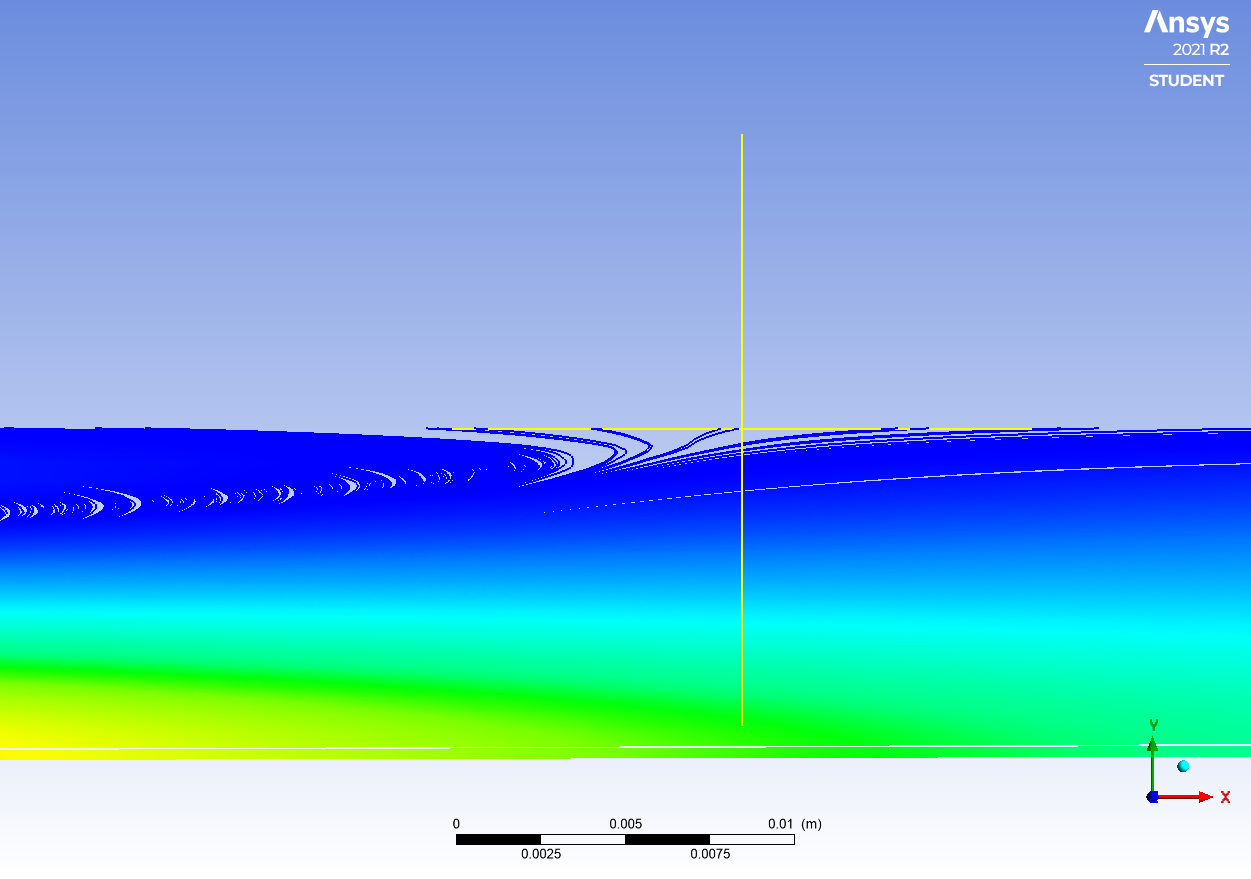
\includegraphics[width=.95\linewidth]{images/task1/100_attachement_0_430.png}
  \subcaption{}
  \label{fig:reat_c}
\end{subfigure}
\hfill
\begin{subfigure}{.75\textwidth}
  \centering
  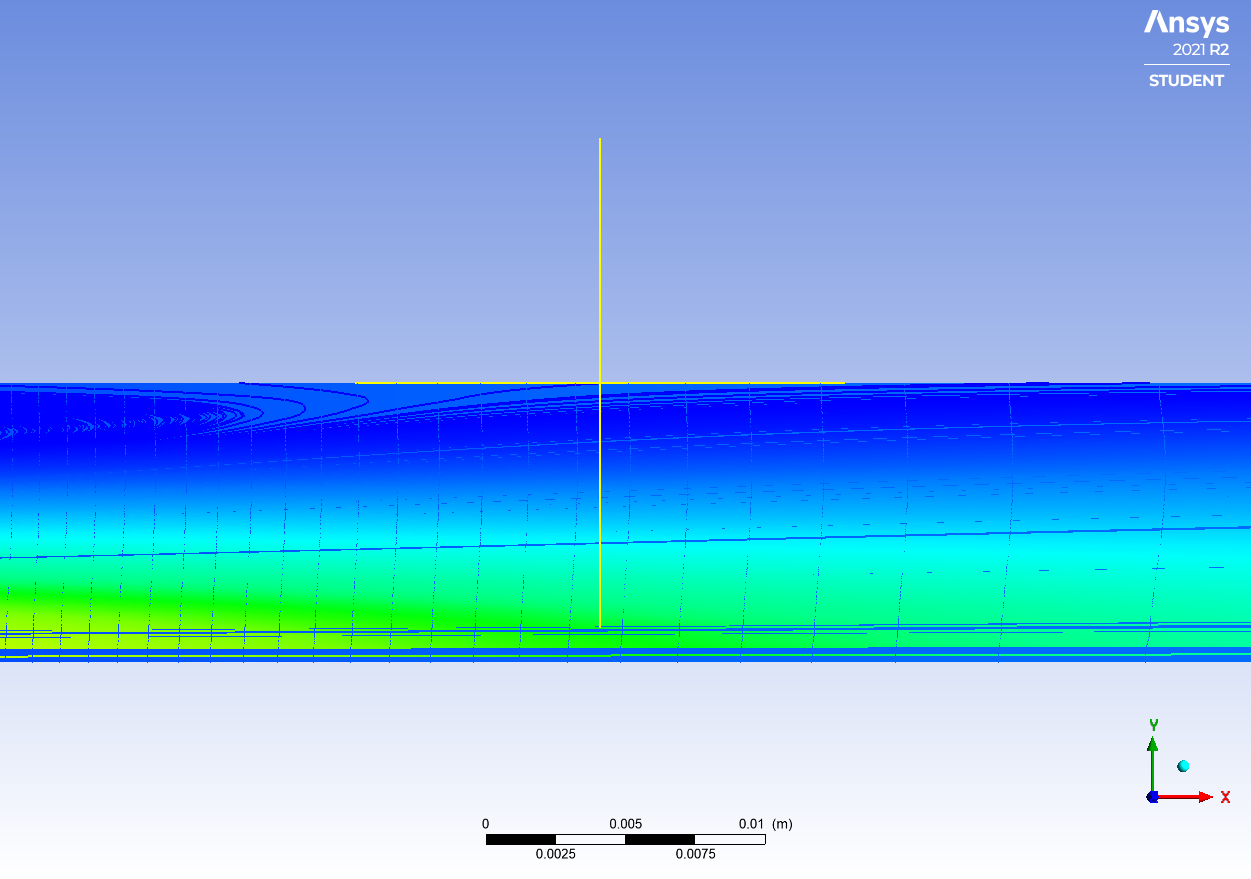
\includegraphics[width=.95\linewidth]{images/task1/150_attachement_0_0681.png}
  \subcaption{}
  \label{fig:reat_d}
\end{subfigure}
\caption{Reattachment Points for 4 different Reynolds numbers.}
\label{fig:reattach}
\end{figure}


